%----------------------------------------------------------------------------------------
%	Einleitung
%----------------------------------------------------------------------------------------

\chapter{Einleitung}
\label{ch:einleitung}
\section{Allgemeines}

\section{Problemstellung}
Die forensische Analyse von digitalen Beweismitteln ist in der heutigen Zeit ein wichtiger Aspekt, um in der Strafverfolgung rechtswidriges Verhalten aufzudecken oder nachzuweisen. In vielen Fällen werden informationstechnische Systeme am Tatort gefunden oder zur Tatbegehung genutzt. Einschlägig sind hierbei Angriffe auf kritische Infrastrukturen durch Computersabotage oder das Ausspähen von Daten. Aber auch Urheberrechtsverletzungen durch die Weitergabe von geschützten Medien oder Verstöße gegen das Wettbewerbsrecht werden mit Informationstechnik begangen.
Je nach Dauer und Umfang der Strafhandlung werden gerade auch im Bereich der Wirtschaftskriminalität dutzende Beweismittel von informationstechnischen Systemen erhoben. Beispielsweise werden beteiligte Computer und Mobiltelefone sichergestellt. Oder es werden logische Sicherungen von Netzwerkspeichern durchgeführt.\\

\noindent
Bei der Analyse dieser Beweismittel möchte ein forensischer Ermittler möglichst schnell einen Überblick über die sichergestellten Daten erhalten. Darauf aufbauend kann er entscheiden, welche Spuren in den Daten zum Nachweis konkreter Tathandlungen dienen und welche potentielle Beweismittel nicht weiter analysiert werden müssen.\\

\noindent
Der kritischste Aspekt hierbei ist, in kürzester Zeit die richtigen Informationen aus allen Daten zu extrahieren. Denn gerade in der Strafverfolgung ist eine schnelle und zielgerichtete Aufarbeitung der Ermittlungsfälle erforderlich. Darüber hinaus werden während der Analyse oftmals weitere Indizien gefunden, welche wiederum zur Sicherung neuer Beweismittel führen können. Je mehr Zeit jedoch für die Analyse benötigt wird, desto höher ist die Gefahr, dass noch nicht sichergestellte Daten endgültig gelöscht werden. Beispielsweise werden Telekommunikationsverbindungsdaten nicht über längere Zeiträume gespeichert.\\

\noindent
Zur Analyse stehen dem Forensiker etliche kommerzielle und Open Source Programme zur Auswahl. Allerdings sind im forensischen Open Source Bereich viele Programme durch die Ressourcen des Analyserechners beschränkt. Sie bieten keine Möglichkeiten rechenintensive Aufgaben performant auf mehreren Computern zu skalieren.\\

\noindent
Aus fachlicher Sicht wäre eine Plattform sinnvoll, die anfallende Analyseaufgaben automatisiert auf allen Daten durchführt. Das System sollte die Ergebnisse unter Berücksichtigung verfügbarer Ressourcen schnellstmöglich ermitteln und dem forensischen Ermittler in einer aufbereiteten Form darstellen. Auf Basis dieser Ergebnisse könnte sich der Forensiker möglichst frühzeitig einen Überblick aller Beweismittel verschaffen, um dann bestimmte Daten und Informationen auch in anderen spezialisierten Analysetools weiterzuverarbeiten. 

\section{Zielsetzung}
Zur Lösung der Problemstellung soll in dieser Masterthesis eine Plattform zur forensischen Analyse entwickelt werden. Diese Plattform soll durch eine automatisierte Analyse und Aufbereitung forensisch relevanter Informationen dem Nutzer helfen, sich einen Überblick zu verschaffen. Der Forensiker soll dadurch effizient und zielgerichtet Datenanalysen durchführen können. Als Basis dieser Plattform soll das Apache Hadoop\textsuperscript{\textregistered} Framework genutzt werden. Hierbei sollen Vor- und Nachteile dieser Art der Datenverarbeitung im forensischen Kontext herausgearbeitet werden.\\ 

\noindent
Apache Hadoop ist ein etabliertes Open Source Framework zur verteilten Speicherung und Verarbeitung von Daten. Durch die Verwendung paralleler Algorithmen eignet sich ein Hadoop-Cluster für große Datenmengen im Terabyte-Bereich. Ein zugrunde liegendes Paradigma ist hierbei, dass die Programmausführung dort stattfindet wo auch die Daten liegen, um kostspielige Datentransporte weitgehend zu vermeiden. Aufgrund dieser Beschaffenheit könnte diese Art der Datenverarbeitung auch Geschwindigkeitsvorteile bei forensischen Analysen bieten. Das Framework selbst besteht aus mehreren Komponenten, welche spezifische Aufgaben der Datenverarbeitung übernehmen. \\

\noindent
Die Basis bildet das verteilte Dateisystem \textit{HDFS}\footnote{HDFS ist die Abkürzung für \textit{Hadoop Distributed File System}.}, welches die Daten redundant auf allen Knoten des Computer-Clusters speichert. Der Zugriff auf die Daten kann über unterschiedliche Komponenten erfolgen.\\
So findet beispielsweise meist Apache Spark\texttrademark\enspace bei der Prozessierung und Analyse der Daten Anwendung. Auch in der Masterthesis soll Apache Spark für anfallende Analysezwecke verwendet werden. Hierbei übernimmt der Ressourcenmanager \textit{YARN}\footnote{YARN ist die Abkürzung für \textit{Yet Another Resource Negotiator}.} die Bereitstellung und Verteilung von verfügbarer Rechenleistung.\\

\noindent
Ein Knackpunkt der Masterthesis ist die Aufbereitung der Daten für die Analyse im Hadoop-Cluster. Beispielsweise könnten die Dateien von sichergestellten Datenträgern direkt in das HDFS kopiert werden. Hierbei muss auf die Unversehrtheit der Dateiinhalte und Metadaten beim Kopieren geachtet werden. \\

\noindent
Im Rahmen dieser Thesis soll die reine Datenanalyse vorerst auf grundlegende Operationen basieren. Unter anderem sollen beispielsweise folgende Informationen zu einzelnen Dateien ermittelt werden: Name, vollständiger Pfad, Hashsumme, Dateityp, Größe, Zeitpunkt der letzten Änderung und Erstellung.\\
Es soll auch eine Volltextsuche auf den Daten möglich sein. Darauf aufbauend soll der Nutzer beispielsweise gleiche Dateien und Verbindungen zwischen den einzelnen Beweismitteln erkennen können.\\
Optional könnte die Analyseplattform gezielt nach IP-Adressen, URLs, E-Mail-Adressen oder Positionsdaten\footnote{Beispielsweise könnten Geopositionen oder Ortsnamen aus Dateien extrahiert werden. Diese Daten könnten dann mit ihrem geografischen Bezug auf einer Karte dargestellt werden.} suchen. Diese Operationen sollen erst implementiert werden, wenn im Rahmen der Thesis noch weitere Bearbeitungszeit vorhanden ist. Sie sind vorerst nicht Gegenstand der Thesis.\\

\noindent
Die Resultate durchgeführter Datenanalysen sollen dem Nutzer bereitgestellt werden. Hierzu soll eine prototypische Implementierung entwickelt werden, deren grafische Oberfläche die fachlichen Aspekte der forensischen Analyse widerspiegelt. Der Forensiker soll Analyseaufgaben konfigurieren und starten können. Nach der Prozessierung soll er die Resultate der Analysen direkt einsehen können.\\
Allerdings ist es nicht das Ziel dieser Thesis, detaillierte Konfigurationsmöglichkeiten und unterschiedlichste Visualisierungen zu implementieren. Dies würde den Rahmen der Arbeit übersteigen. Der Fokus dieser Fachanwendung liegt bei der schlichten Anzeige der Analyseergebnisse. In diesem Kontext soll auch geprüft werden, ob existierende Programme zur Datenvisualisierung im Hadoop-Umfeld wiederverwendet werden können.\\

\noindent
Nachfolgende Abbildung soll den den groben Aufbau dieser Plattform skizzieren. Der Forensiker importiert die forensischen Rohdaten in das Hadoop-Cluster. Darauf hat er die Möglichkeit diverse Analysen auf den Daten durchzuführen. Zuletzt kann er die Ergebnisse über eine entsprechende Oberfläche einsehen und hat die Möglichkeit die Daten innerhalb oder außerhalb des Hadoop-Clusters weiterzuverarbeiten.\\

\begin{figure}[ht]
  \centering
  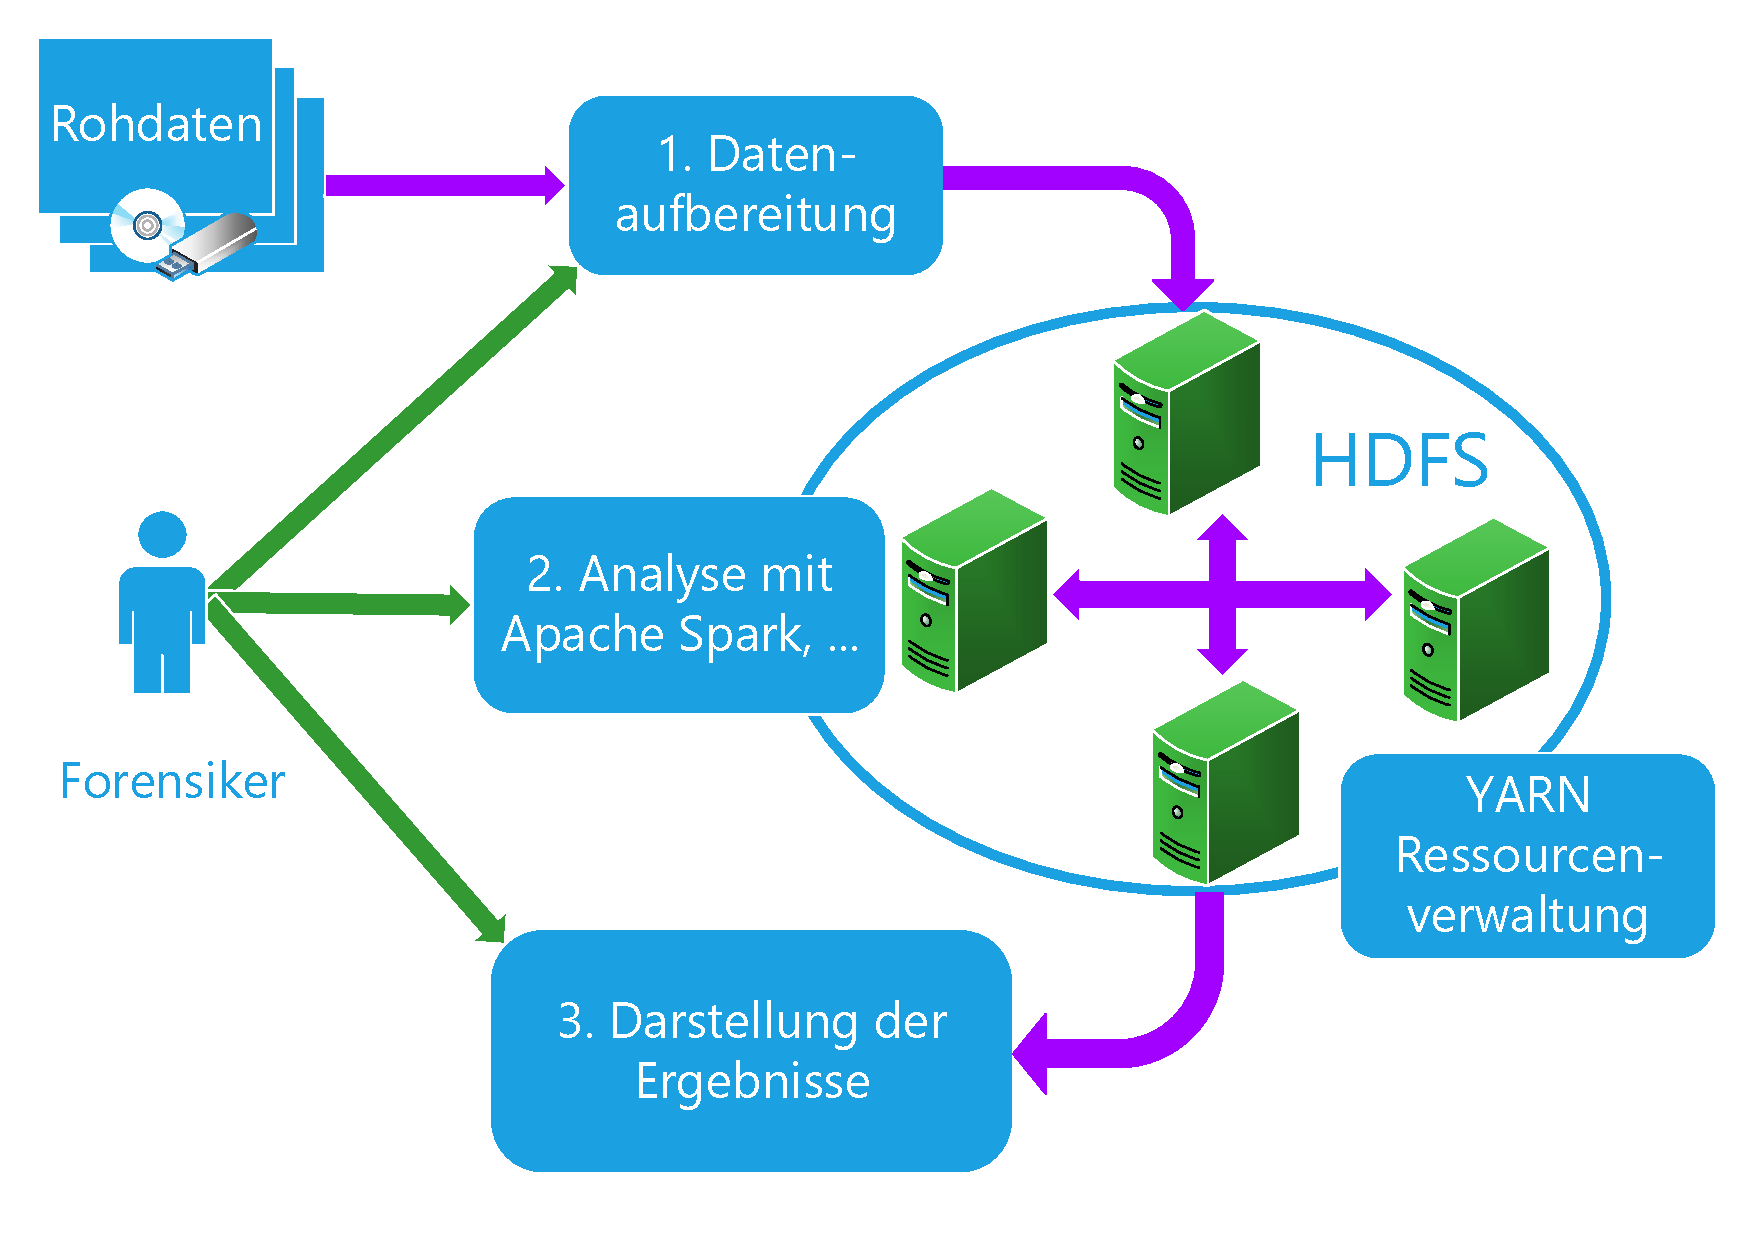
\includegraphics[width=0.82\textwidth]{./resource/Hadoop-Struktur.pdf}
  \caption{Datenverarbeitung im Hadoop-Umfeld}
\end{figure}

\noindent
Das Ziel dieser Masterthesis ist es, dem forensischen Ermittler schnellstmöglich einen Überblick zu den einzelnen Beweismitteln und deren Zusammenhänge im Kontext einer Fallanalyse zu liefern. 

\section{Weitere Aspekte der Thesis}
Bei einer realen forensischen Analyse gibt es weitere Anforderungen, die das Analysesystem erfüllen sollte. Im Rahmen der Masterthesis soll geprüft werden, ob diese Anforderungen durch die Nutzung des Apache Hadoop Frameworks abgedeckt werden und welche technischen oder organisatorischen Regelungen getroffen werden müssen.\\
Das System muss gegen fremden Zugriff gesichert sein. Es muss zu jeder Zeit ersichtlich sein, welche Personen zu welchem Zweck auf das System zugreifen.\\

\noindent
Da in vielen Fällen hochsensible personenbezogene Daten und Geschäftsgeheimnisse verarbeitet werden, müssen auch entsprechende Regelungen getroffen werden, wie nach der Analyse alle Daten restlos aus dem System gelöscht werden können.\\

\noindent
Ein weiterer Aspekt in der Analyse ist die lückenlose Erstellung einer Beweismittelkette (Chain of Custody). Für jedes forensische Analyseergebnis müssen die Herkunft und die Verarbeitungsschritte transparent nachvollziehbar sein. \\

\noindent
Auch die Korrektheit der Analyseergebnisse muss verifiziert werden. Hierfür sollen im Rahmen der Masterthesis entsprechende Testdaten erstellt oder beschafft werden, welche die Funktionsfähigkeit der Plattform prüfen. \\

\noindent
Aus organisatorischer Sicht soll die Analyseplattform als Open Source Projekt bereitgestellt werden. Hierzu soll der Source-Code, die Konfiguration des Systems und die Dokumentation in einem öffentlich zugänglichen Repository verfügbar sein.\footnote{Sicherheitskritische Informationen, wie beispielsweise Zugangsdaten, müssen unkenntlich gemacht werden.}


\section{Aufbau}
In Kapitel \ref{ch:einleitung} wird die grundlegende Problemstellung bei der forensischen Analyse beschrieben, welche diese Masterthesis lösen soll. Darauf folgt die Zielsetzung der Thesis, welche als möglicher Lösungsvorschlag zur beschriebenen Problemstellung gilt.\\
In Kapitel \ref{ch:development_approach} folgt das allgemeine Entwicklungsvorgehen. Darin ist auch der aktuelle Projektplan enthalten, welche die Arbeitspakete definiert.
Zusätzlich wird der Umgang mit Quellcode und Konfigurationsdateien als Open-Source Projekt beschrieben.\\

\noindent
In Kapitel \ref{ch:theory_hadoop} erfolgt eine Darstellung der Apache Hadoop Plattform inklusive theoretischen Grundlagen zur Arbeitsweise des Frameworks. Des Weiteren werden darauf aufbauend Projekte Apache Spark, Apache Hive und Apache HBase und deren Einsatzbereiche erläutert.\\

\noindent
In Kapitel \ref{ch:praxis_analysis} werden die angewendeten Tools für eine herkömmliche fachliche Analyse eines Beweismittels beschrieben. Parallel hierzu wird bei jedem herkömmlichen Programm geprüft, wie das gleiche Ergebnis mit der Analyseplattform erzielt werden kann. Diese Kapitel soll sozusagen die Überleitung von der herkömmlichen Analyse auf einem Computer hin zu Analyse im Hadoop-Cluster beschrieben. Als Ergebnis soll anschaulich dargestellt werden, welche fachliche Analyse-Schritte mithilfe eines Hadoop-Cluster sinnvoll und performant durchgeführt werden können.\\

\noindent
Zuletzt erfolgt in Kapitel \ref{ch:zusammenfassung} eine Zusammenfassung der erarbeiteten Ergebnisse. Offene Punkte und Verbesserungen des Systems werden in Kapitel \ref{ch:ausblick} diskutiert. 
